\section{Operator}
\label{sec:komponenten:operator}

Operatoren oder auch Controller genannt, bieten die Möglichkeit, die Kubernetes API mit eigenen Typen und Funktionen zu erweitern.
Eigene Typen beziehungsweise \acp{CR} werden mittels einer \ac{CRD} erweitert.
\begin{figure}[h]
  \centering
  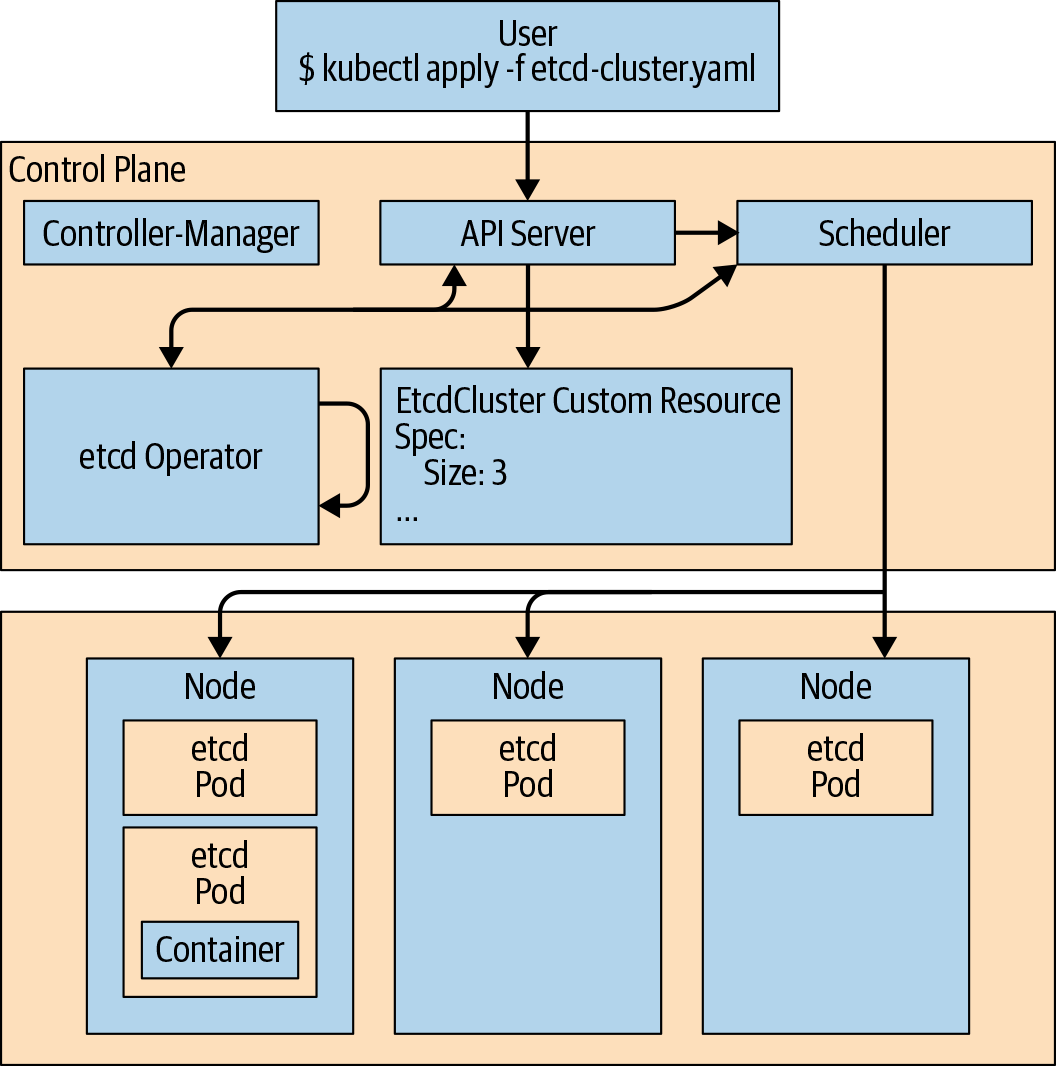
\includegraphics{gfx/chapters/3_komponenten/operator_example.png}
  \caption{Funktionen eines Kubernetes Operators}
  \source{\cite{Dobies2020}}
  \label{fig:kubernetes_operator_example}
\end{figure}

In \ref{fig:kubernetes_operator_example} wird dargestellt, wie ein Kubernetes Operator funktioniert. Der Operator läuft im Cluster und
überwacht den API-Server auf Änderungen seiner \ac{CR} und ergreift auf Grundlage des Zustands der Ressource Maßnahmen im Cluster, 
wie beispielsweise das Erstellen neuer Pods. \cite{Dobies2020}
Diesen Synchronisationsmechanismus nennt man \emph{Reconciliation}.

Der Operator für die Referenzimplementation des Chat \ac{SaaS} nutzt diesen Synchronisationsmechanismus, um die Erstellung des RocketChat
Deployments zu vereinfachen. Der Rocket API Server erstellt eine \ac{CR} Ressource im Cluster und kümmert sich nicht weiter um 
das Deployment. Operatoren können sich zusätzlich zum Deployment und der Konfiguration auch um die Funktionen Backup 
und automatische Reperatur des Services kümmern \cite{Dobies2020}, welche allerdings in dieser Referenzimplementation 
nicht berücksichtigt wurden.

Rocket.Chat besteht im Deployment aus einer MongoDB\footnote{\href{https://www.mongodb.com/}{MongoDB}}, welche als Replicaset konfiguriert wird,
sowie dem eigentlichen Webserver, welcher als Endpunkt für Clients dient.

Die Bereitstellung des Chat Services besteht aus den folgenden Kubernetes Ressourcen \ref{subsec:kubernetes:ressourcen}:
\begin{itemize}
  \item ConfigMap für MongoDB Scripts
  \item Secret für MongoDB Authentifizierung (Username und Passwort)
  \item Persistent Volume für MongoDB
  \item Service für Rocket.Chat und MongoDB Pods
  \item Deployment für Rocket.Chat Pods
  \item StatefulSet für MongoDB Pods
  \item Ingress für Rocket.Chat
  \item ServiceAccount
\end{itemize} 

Hierbei werden Änderungen an dem erstellten Rocket \ac{CR} von der Kubernetes API an den Operator weitergegeben, um
notwendige Anpassungen an das Deployment zu machen, beispielsweise falls sich eine Containerimageversion ändert 
oder die Ressource gelöscht wird. 

\subsection{Rocket Custom Resource}
Als API für den Operator dient die Rocket Chat \ac{CRD}. Diese wird im Code als Go Struct definiert, welches letztendlich
als JSON\footnote{\href{https://www.json.org/json-de.html}{JSON}} Objekt an die Kubernetes API gesendet wird.
Genauer dargestellt wird die Ressource in \ref{chap:rocketchat_crd_spec}, in dem aufgezeigt wird, wie das Objekt aufgebaut ist.
Nutzer des Kubernetes Cluster können selbst solche Rocket \acp{CR} via YAML oder JSON Dateien erstellen und
an die Kubernetes API schicken. Für diese \ac{SaaS} Anwendung ist dieser Anwendungsfall allerdings nicht vorgesehen.
Endnutzer sollen sich nicht mit der Thematik von Kubernetes auseinander setzen müssen, 
sondern nur per Konfiguratorclient (\ac{CLI} oder Webinterface) ihren Chat Service erstellen.


